\documentclass[a4paper]{article}
\usepackage[utf8]{inputenc}
\usepackage[T1]{fontenc}
\usepackage[francais]{babel}
\usepackage{graphicx}
\usepackage[a4paper]{geometry}
\usepackage{amsmath,amsfonts,amssymb}
\usepackage{stmaryrd}
\usepackage{algorithm}
\usepackage{tikz}
\usepackage[noend]{algpseudocode}
\geometry{hscale=0.7,vscale=0.7,centering}
\usepackage{float}

\makeatletter
\def\BState{\State\hskip-\ALG@thistlm}
\makeatother

\begin{document}
\newcommand\tab[1][1cm]{\hspace*{#1}}
\newcommand\spc[1][0.1cm]{\hspace*{#1}}
\title{
        \includegraphics[scale=3]{ULBsciences_droit}\\
        Projet: Les bons comptes font les bons amis \\
      }
\author{
David Majcherczyk,Kishiro Nishio\\
Facult\'e des Sciences, Universit\'e Libre de Bruxelles\\
}
\date{2016-2017}
\maketitle
\thispagestyle{empty}
\newpage
\setcounter{page}{1}
\section{Introduction}
L'emprunt et ainsi la création de dettes est un phénomène courant dans la société. Le projet a pour objectif la conception d'un programme mémorisant et simplifiant les dettes au sein de communautés.

\section{description et tests}
\subsection{Structure du programme}
Le programme se compose de plusieurs classes de manière à suivre le paradigme orienté objet .Le rôle chaque classes est expliqué ci dessous. Le main se situe dans lbcflba.py, la création du graphe suivie des autres algorithmes demandés y est lancée.  
\smallbreak
\noindent Classes:
\begin{itemize} 
\item Graph: Cette classe représente le graphe en lui même, Il a pour attribut la liste des noeuds du graphe, mais les liens entre ces noeuds(arcs) ne s'y trouvent pas. Il possède également la liste des communautés qui le composent ainsi que la liste des hubs sociaux qui articulent ce graphe. Les méthodes de création, de simplification du graphe, d'identification des communautés et d'identification des hubs s'y trouvent également.
\item Node: L'attribut de l'objet Graph qui contient la liste de noeuds est logiquement une liste composée d'objet Noeuds. C'est dans cet objet que l'on trouve les liens vers les autres objets "Node". Ce lien est représenté par une liste d'Arcs. En plus, cet attribut on retrouve également le nom, la position dans le graphe(ordre d'arrivé, utilisé dans la recherche de composantes fortements connexes) et pour finir un booléen indiquant si le noeud se trouve dans une comunauté(utilisé ds la recherche de communautés). Les méthodes sont pour la plupart des getters/setters. En plus de celles-ci, on y trouve la méthode permettant d'ajouter un arc. 
\item Arc: Cet objet compose la liste dans "Node". Il n'a que deux attributs, "extremite" qui est de type "Node". Extremité est donc le sommet qui se trouve au bout de l'arc. Ainsi, on peut parcourir le graphe en passant de sommet à sommet par l'intermédiaire d'arcs. Le deuxième attribut est le poids de l'arc. Dans notre contexte, il correspond à la dette entre la personne dont part l'arc et la personne à l'"extremité" de l'arc.
\item Cfc: Composante fortement connexe. Les méthodes servent principalement à la suppresion de cycles.
\item Community: = 1 Communauté. Chaque communauté possède un id utilisé dans l'algorithme de recherche de communautés.   
\end{itemize}
\newpage
\subsection{Présentation des tests}
\subsubsection*{Test 1}
Le premier graphe testé est celui fourni dans l'énoncé.
\subsubsection*{Test 2}
Le deuxième test est un graphe conçu pour vérifier qu'il n'y a pas de simplification si il n'y pas de cycle.
\bigbreak
\begin{tikzpicture}
\node () at (0,0) {};
\node[shape = circle,draw=black](A) at (4,-0.75) {A};
\node[shape = circle,draw=black](B) at (6,-0.75) {B};
\node[shape = circle,draw=black](C) at (8,-0.75) {C};

\path [->] (A) edge[anchor = south] node {$10$} (B);
\path [->] (B) edge[anchor = south] node {$5$} (C);
\end{tikzpicture}
\subsubsection*{Test 3}
Le troisième test est un graphe conçu pour vérifier que la simplification de cycle se fait plusieurs fois si il en reste après la première simplification.

\begin{tikzpicture}
\node () at (0,0) {};
\node[shape = circle,draw=black](A) at (5,-0.75) {A};
\node[shape = circle,draw=black](B) at (7,-0.75) {B};
\node[shape = circle,draw=black](D) at (5,-2.75) {D};
\node[shape = circle,draw=black](C) at (7,-2.75) {C};

\path [->] (A) edge[anchor = south] node {$20$} (B);
\path [->] (B) edge[anchor = west] node {$10$} (C);
\path [->] (C) edge[anchor = south] node {$15$} (D);
\path [->] (B) edge[anchor = south east] node {$5$} (D);
\path [->] (D) edge[anchor = east] node {$40$} (A);
\end{tikzpicture}

\subsubsection*{Test 4}
Le quatrième test est un graphe conçu pour vérifier que la concaténation de communauté se fait bien pour notre algorithme.

\begin{tikzpicture}
\node () at (0,0) {};
\node[shape = circle,draw=black](A) at (4,-0.75) {A};
\node[shape = circle,draw=black](B) at (6,-0.75) {B};
\node[shape = circle,draw=black](C) at (8,-0.75) {C};
\node[shape = circle,draw=black](D) at (4,-2.75) {D};
\node[shape = circle,draw=black](E) at (6,-2.75) {E};

\path [->] (B) edge[anchor = south] node {$20$} (C);
\path [->] (B) edge[anchor = west] node {$10$} (E);
\path [->] (A) edge[anchor = east] node {$15$} (D);
\path [->] (D) edge[anchor = north] node {$40$} (E);
\end{tikzpicture}
\newpage 
\subsection{Parsing}
\subsubsection{createGraph()}
Le rôle de cet algorithme est d'extraire les informations nécessaires à la création du graphe. Cela se fait ligne par ligne. Des opérations telles que les splits sont nécessaires pour "épurer" la ligne. La création du graphe se fait ligne par ligne en appelant updateGraphe.
\begin{algorithm}
\caption{createGraph}\label{createGraph()}
\begin{algorithmic}[1]
\Procedure{createGraph}{$fileName$}
\BState \emph{try}:
\State \textbf{Ouverture} \text{du fichier} \textbf{fileName}
\State $ \textit{\_graphOrder} \gets \text{lecture première ligne}$
\BState \emph{except}:
\State $\text{Print erreur}$
\For{$\text{chaque ligne après la première}$}
\State $\text{strip split(" ")}$
\State $\textit{firstPerson} \gets \text{premier caractère ou chaîne(différent de " ") récupéré de la ligne }$
\State $\textit{secondPerson} \gets \text{deuxième caractère ou chaîne("différent de " ") récupéré de la ligne}$
\State $\textit{debt} \gets \text{nombre récupéré de la ligne}$
\State \textbf{updateGraph}\text{(}\textit{firstPerson,secondPerson,debt}\text{)} \text{Voir} Algorithm~\ref{updateGraph()}
\EndFor
\State \textbf{Fermeture} \text{du fichier}
\EndProcedure
\end{algorithmic}	
\end{algorithm}
\begin{figure}[H]
%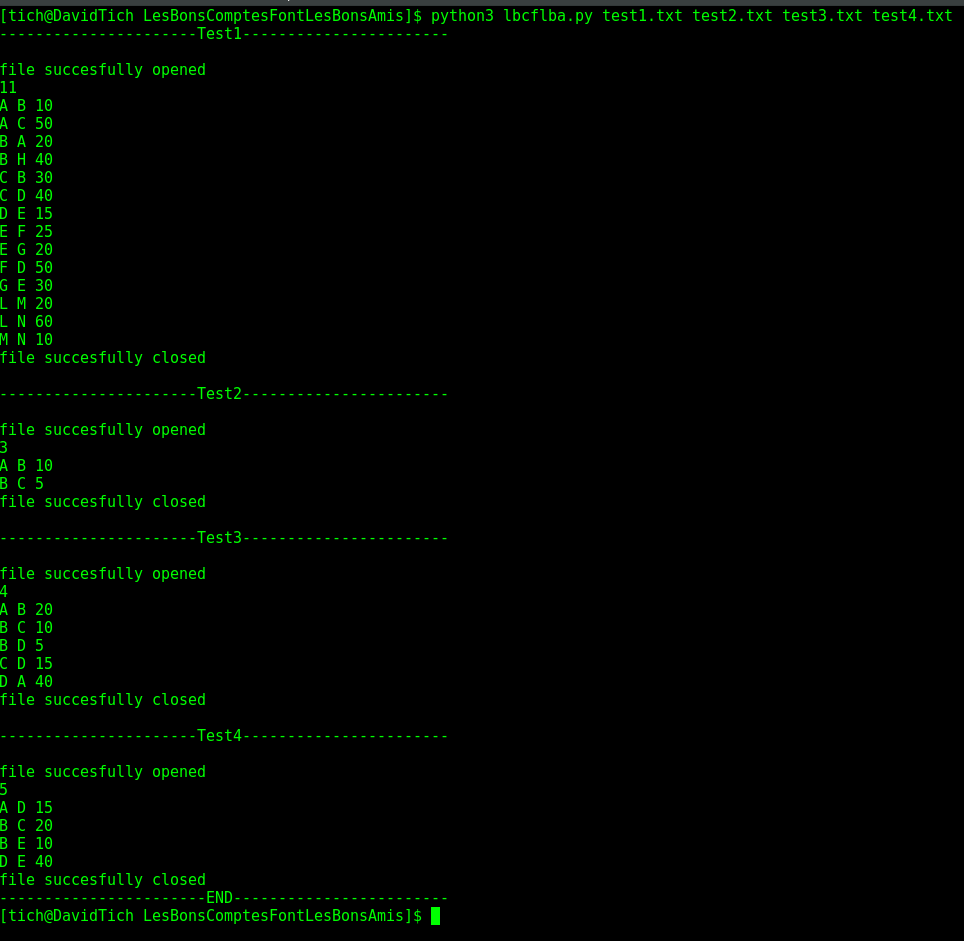
\includegraphics[scale=0.4]{createGraph.png}\\
\end{figure}
\newpage
\subsubsection{updateGraph()}
La création du graphe se fait donc ligne par ligne. L'algorithme met à jour l'ancienne version du graphe à chaque fois qu'il est appelé. La construction du graphe est finalisée lorsqu'il ne reste plus de ligne dans le fichier.

La mise à jour se fait comme ceci:
\begin{enumerate}
\item On regarde si les personnes sont déjà dans le graphe.
\item \begin{enumerate}
\item Une des deux ou les deux personnes ne sont pas présentes. Dans ce cas, on crée un objet "Node" (qui représente une personne dans le graphe) pour chaque persone qui n'est pas encore dans le graphe.
\item Les 2 sont présentes. On simplifie les dettes entre elles(cancelMutualDebt). Ceci évite de devoir reparcourir plus tard. 
\end{enumerate}
\item Création et ajout de l'arc allant de la première à la deuxième personne dans le "Node" de la première personne. On va de la première à la 2ème puisque c'est cette relation qui est décrite dans le fichier.
\end{enumerate}
\begin{algorithm}[H]
\caption{updateGraph}\label{updateGraph()}
\begin{algorithmic}[1]
\Procedure{updateGraph}{$fPerson,sPerson,debt$}
\State $\textit{fPresent} \gets \text{initialisé à 0} $ \Comment{f pour first s pour second}
\State $\textit{sPresent} \gets \text{initialisé à 0} $
\Comment{variables indiquant si la 1ère et 2ème personne sont déjà dans le graphe en construction}
\While{$\textit{(fPresent} \textbf{ ou } \textit{sPresent == 0) } \textbf{and } \textit{i}\text{ < nb de noeuds déjà dans le graphe}$} \label{While}
\If{\textit{fPerson} \text{== 0} \textbf{and} \textit{fPerson} == \text{self.nodes[}\textit{i}\text{].}\textbf{getName()} }
\State $\textit{fPerson} \gets \text{1 (marqué que la personne est trouvée)}$
\State $\textit{nodeF} \gets \text{self.nodes[i]}$
\EndIf
\If{\textit{sPerson} \text{== 0} \textbf{and} \textit{sPerson} == \text{self.nodes[}\textit{i}\text{].}\textbf{getName()} }
\State $\textit{sPerson} \gets \text{1 (marqué que la personne est trouvée)}$
\State $\textit{nodeS} \gets \text{self.nodes[i]}$
\EndIf
\EndWhile
\If{\textit{fPresent == 0(pas encore dans le graphe)}} 
\State $\textit{nodeF} \gets \textbf{Node}\text{(}\textit{fPerson,len(self.nodes)\text{)}} $
\State $\text{self.node.append(}\textit{nodeF}\text{)}$
\EndIf
\If{\textit{sPresent == 0(pas encore dans le graphe)}} 
\State $\textit{nodeS} \gets \textbf{Node}\text{(}\textit{sPerson,len(self.nodes)\text{)}} $
\State $\text{self.nodes.append(}\textit{nodeS}\text{)}$
\EndIf
\If{\textit{fPresent} \text{== 1} \textbf{and} \textit{sPresent} \text{== 1}\textit{(tous les 2 déjà présents)}} 
\State $\textit{debt} \gets \textbf{cancelMutualDebt}\text{(}\textit{nodeF,nodeS,debt}\text{)} $ \text{Voir} Algorithm~\ref{cancelMutualDebt}
\EndIf
\State $\textit{newArc} \gets \textbf{Arc}\textit{(nodeS,debt)}$
\State $\textit{nodeF.}\textbf{addArc.}\textit{(newArc)} $    	
\EndProcedure
\end{algorithmic}
\end{algorithm}

L'attribut self.nodes est la liste contenant tous les noeuds du graphe. Elle est ici en construction. les noeuds sont de type "Node".

Operation~\ref{While} : La première partie de la condition sert à détecter si les noeuds font déjà partis du graphe en construction et la deuxième sert à s'arrêter au bout du graphe en construction si les 2 ou 1 des 2 noeuds n'y est pas encore.(s'arrête plutot si les 2 sont trouvés)

Pour ce test, On montre que les sommets sont bien tous ajoutés au graphe. Montrer les liens entre ces sommets prendrait trop de place.
\begin{figure}[H]
%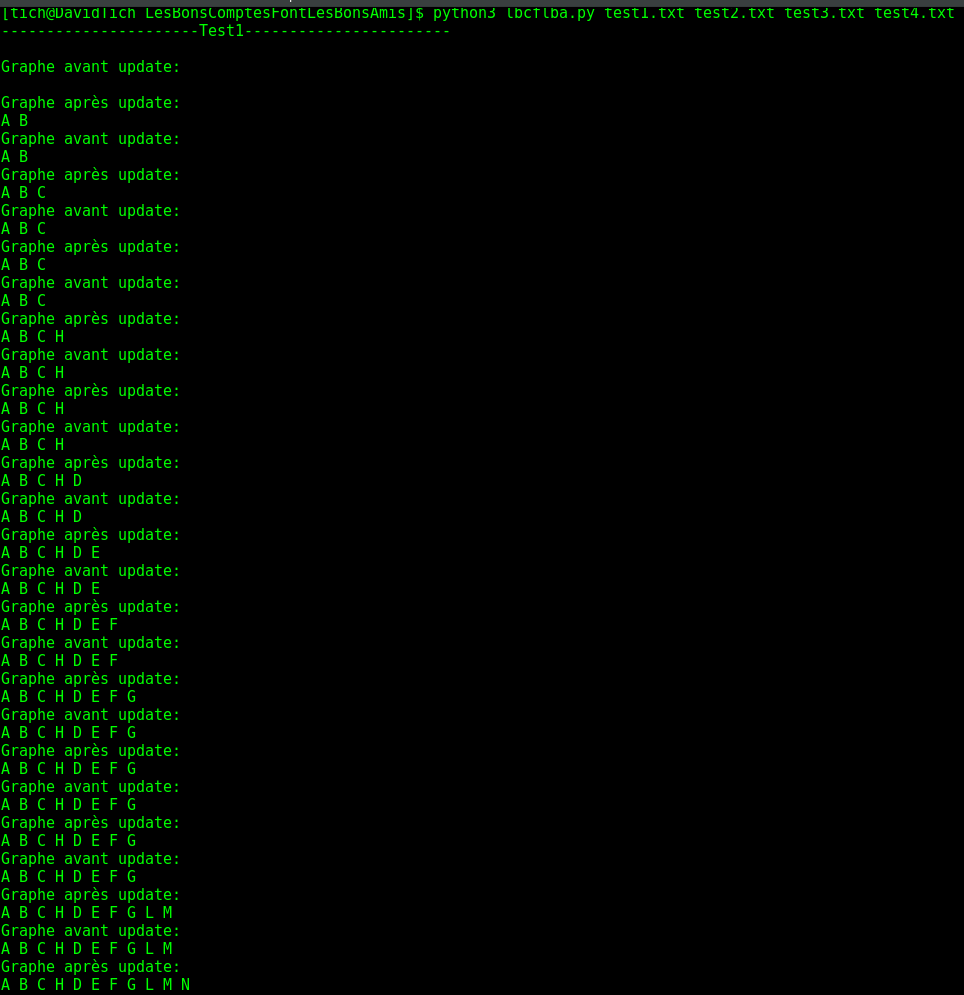
\includegraphics[scale=0.4]{update1.png}\\
\end{figure}
\begin{figure}[H]
%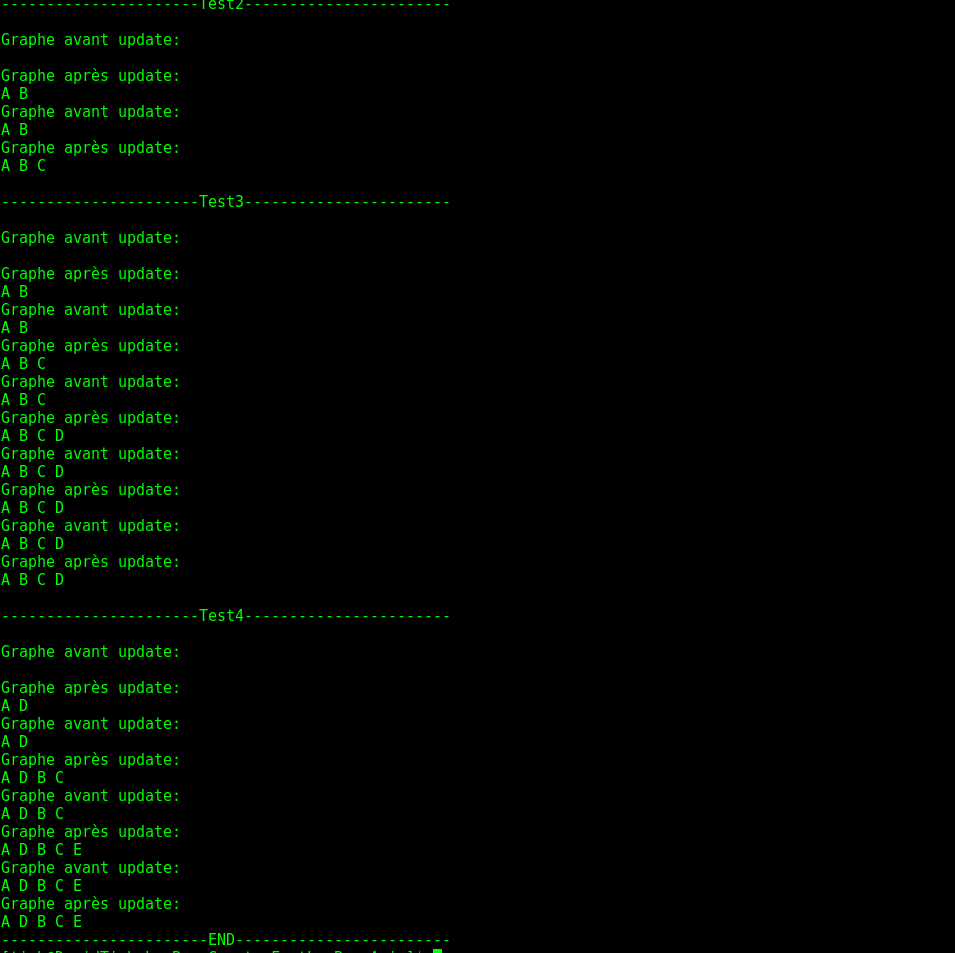
\includegraphics[scale=0.4]{update2.png}\\
\end{figure}	
\subsubsection{cancelMutualDebt()}
Cet algorithme permet donc de simplifier les dettes entre 2 noeuds. Si ils se doivent mutuellement de l'argent.

Etapes:
\begin{enumerate}
\item On parcourt les arcs de la 2 ème personne jusqu'à trouver celui qui va vers la première personne.(l'arc de la première vers la 2 ème est celui fourni à la ligne du fichier qui est entrain d'être ajoutée dans le graphe)
\item On soustrait la plus grande dette à la plus petite. On place donc la différence entre les 2 poids dans l'arc avec le poids le plus élevé et 0 dans le plus petit.
\end{enumerate}
\begin{algorithm}[H]
\caption{cancelMutualDebt}\label{cancelMutualDebt}
\begin{algorithmic}[1]
\Procedure{cancelMutualDebt}{$nodeS,nodeF,debtSF$}
\For{\textit{arc}\text{ dans la liste des arcs partant de nodeS}}
\If{ \text{Sommet à l'extrémité de} \textit{arc} \text{==} \textit{nodeF}}
\State $\textit{debtSF} \gets \text{ poids de } \textit{arc}$
\If{$\textit{ debtSF} \leq \textit{debtFS}$ }
\State \textit{arc.}\textbf{setPoids}\textit{.(debtSF-debtFS)}
\State \text{return 0}
\Else
\State \textit{arc.}\textbf{setPoids}\text{.(0)}
\State \text{return} \textit{(debtFS-debtSF)}
\EndIf
\EndIf
\EndFor
\State{\text{return} \textit{debtFS}}
\EndProcedure
\end{algorithmic}
\end{algorithm}
Pour cette partie seul le test1 est pertinent.
\begin{figure}[H]
%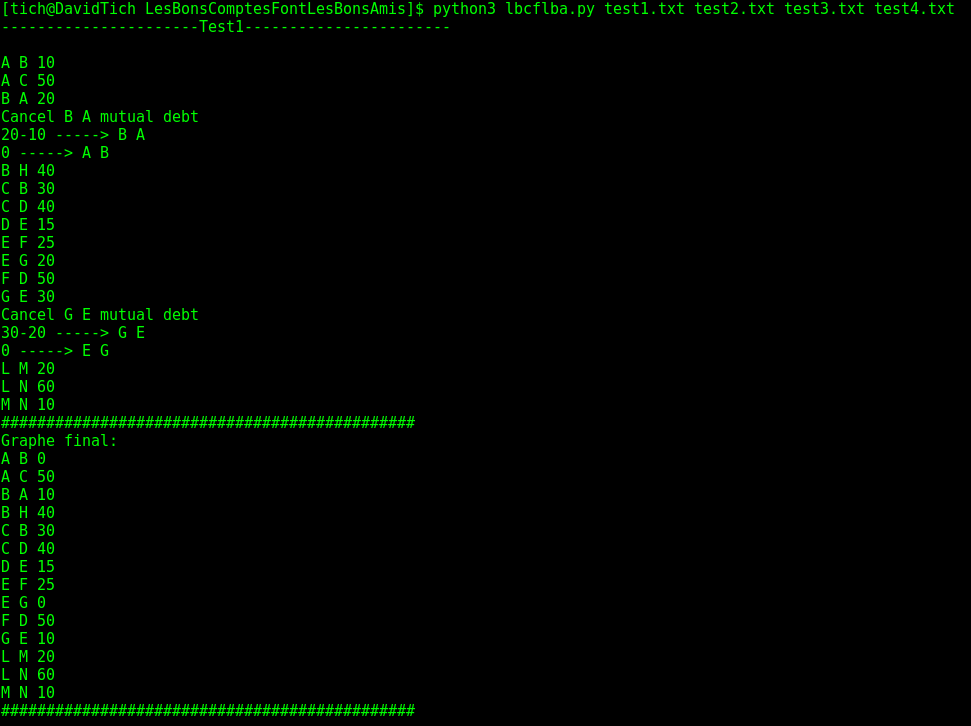
\includegraphics[scale=0.4]{cancel.png}\\
\end{figure}
\subsection{Simplification des dettes [classe: Graph]}
Il y a plusieurs étapes répartie en 2 classes pour la simplification.

Pour la classe Graph:
\begin{enumerate}
\item On trouve les composantes fortement connexes à l'aide de l'algorithme du cours. Ces composantes sont sous forme brute.(findCfc)
\item On transforme ces données pour obtenir des listes de composantes avec les indices des sommets. On construit ensuite les objets "Cfc" pour chaque composante existante. Ces objets ont pour but de pouvoir effectuer des opérations sur les composantes fortements connexes facilement.(saveCFCGreaterThenOne) Important: On ne retient que les composantes fortement connexes ayant plus d'un sommet.
\item Suppression des cycles.
\end{enumerate}
\subsubsection{simplific()}
Cette méthode sert uniquement à appeler les méthodes qui réalise les étapes citées plus haut. Elle le fait tant qu'il reste des CFCs
\begin{algorithm}[H]
\caption{simplific}\label{simplific}
\begin{algorithmic}[1]
\Procedure{simplific()}{}
\State \textbf{findCFC()}
\State \textbf{saveCFCGreaterThenOne()}
\State \textbf{deleteCycles()}
\While{ \text{il y a encore au moins une composante fortement connexe de taille supérieure à 1}}
\State \textbf{findCFC()}
\State \textbf{saveCFCGreaterThenOne()}
\State \textbf{deleteCycles()}
\EndWhile
\EndProcedure
\end{algorithmic}
\end{algorithm}
\subsubsection{findCFC()}
Cet algorithme parcourt les sommets du graphe à la recherche de sommets non marqués et si tel est le cas, appelle la méthode explore en donnant en paramètre l'index du sommet.
\begin{algorithm}[H]
\caption{findCFC()}\label{findCFC}
\begin{algorithmic}[1]
\Procedure{findCFC()}{}
\State $\textit{id}\gets \text{0}$
\State $\textit{sid}\gets \text{0}$
\For{\text{les sommets du graphe}}
\State $\textit{pre[sommet]}\gets \text{-1}$
\State $\textit{low[sommet]}\gets \text{0}$
\State $\textit{comp[sommet]}\gets \text{0}$
\EndFor
\For{\text{les sommets du graphe}}
\If{\text{le sommet n'est pas marqué}}
\State \textbf{self.exploreCC}\text{(index du sommet courant)}
\EndIf
\EndFor
\EndProcedure
\end{algorithmic}
\end{algorithm}
\subsubsection{explore()}
Cet algorithme fait presque la meme chose que \textit{exploreCC} (CF:2.7.2) à la difference qu'au lieu de retourner la valeur minimum, il stocke celle-ci dans \textit{low}. Et c'est cette  même liste \textit{low} qui va permettre la détection d'arcs de retour.Si on ne detecte pas d'arcs de retour pour le sommet courant, c'est que celui-ci fait donc partie d'une autre composante fortement connexe que ceux précédemment rencontrés.
\begin{algorithm}[H]
\caption{explore}\label{explore}
\begin{algorithmic}[1]
\Procedure{explore}{(k)}
\State $\textit{id} \gets \textid{id}\text{ + 1} $
\State $\textit{pre[k]} \gets \textit{id} $
\State $\textit{low[k]} \gets \textit{id} $
\State $\textit{minimum} \gets \textid{id} $
\State $\textit{stack}\text{.append(k)} $
\For{\textit{i}\text{ pour tous les arcs de }\textit{nodesNames[k]}}
\If{\text{l'arc courant}\textit{i}\text{a une dette}}
\State $\textit{t}\gets \textit{i}\textbf{.getExtremite().getPosition()}$
\If{\textit{pre[t]}\text{ n'est pas marqué}}
\State $\textbf{self.explore(t)}$
\EndIf
\If{\textit{low[t]}\text{ est plus petit que }\textit{minimum}}
\State $\textit{minimum}\gets \textit{low[t]}$
\EndIf
\EndIf
\EndFor
\If{\text{le minimum resultant }\textit{m}\text{ est plus grand que la valeur à l'indice }\textit{k}\text{ de }\textit{low}}
\State $\textit{low[k]}\gets \textit{minimum}$
\EndIf
\Else
\State $\textit{t}\gets \textit{stack}\textbf{.pop()}$
\State $\textit{comp[t]}\gets \textit{sid}$
\State $\textit{low[t]}\gets \text{100000000}$
\While{ \textit{t}\text{ est différent de }\textit{k}}
\State $\textit{t}\gets \textit{stack}\textbf{.pop()}$
\State $\textit{comp[t]}\gets \textit{sid}$
\State $\textit{low[t]}\gets \text{100000000}$
\EndWhile
\State $\textit{comp[t]}\gets \textit{sid}$
\State $\textit{sid}\gets \textit{sid + 1}$
\EndIf
\EndProcedure
\end{algorithmic}
\end{algorithm}


\subsubsection{saveCFCGreaterThenOne()}
\begin{algorithm}[H]
\caption{saveCFCGreaterThenOne}\label{save}
\begin{algorithmic}[1]
\Procedure{saveCFCGreaterThenOne}{}
\State $\textit{self.CFCs} \gets \text{ [] initialisation attribut qui va contenir les cfcs} $
\State $\textit{temp} \gets \text{ []} $
\For{\text{i de 0 à ordre du graphe}}
\If{\text{longueur de }\textit{temp}\text{-1 < numéro de la composante dans} \textit{self.comp} \text{à l'indice} \textit{i}}
\For{\text{numéro de la composante - longueur}\textit{ temp}\text{-1}}
\State $\textit{temp}\text{.append([])}$
\EndFor
\EndIf
\State $\textit{temp}\text{[numéro de la composante].append(}\textit{i}\text{)}$
\EndFor
\For{\text{k de 0 à longueur de}\textit{ temp}}
\If{$\text{longueur de }\textit{temp}\text{[k] > 1}$}
\State $\textit{tempCfc} \gets \textbf{Cfc}\text{(premier sommet de la composante}\textit{ k}\text{)}$
\For{\textit{l}\text{ de 0 à (longueur composante }\textit{k}\text{)-1}}
\State \textit{tempCfc}\textbf{.addSummit}\text{(sommet }\textit{l}\text{+1 dans la composante)}
\EndFor
\State \textit{self.CFCs}\text{append(tempCfc)}
\State \textit{self.CFCs}$\text{[dernier élémént de CFCs que l'on vient d'ajouter]}$\textbf{.getLinkingArcs()}
\State \textit{self.CFCs}$\text{[dernier élémént de CFCs que l'on vient d'ajouter]}$\textbf{.initMarkedList()}
\EndIf
\EndFor
\EndProcedure
\end{algorithmic}
\end{algorithm}
\subsubsection{deleteCycles}
Appel à la suppression des cycles pour toutes les CFC >1.
\begin{algorithm}
\caption{deleteCycles}\label{delete}
\begin{algorithmic}[1]
\Procedure{deleteCycles()}{}
\For{\textit{i}\text{ de 0 à longueur de }\textit{self.CFCs}}
\State $\textit{self.CFCs}\text{[}\textit{i}\text{]}\textbf{.deleteCycle()}$
\EndFor
\EndProcedure
\end{algorithmic}
\end{algorithm}
\subsection{Simplification des dettes [classe: CFC]}
\subsubsection{getLinkingArcs()}
Une fois que l'on a les sommets on a besoin des Arcs qui les lient. On retient également le  sommet avec le poids le plus faible(pour notre algorithme de suppresion de cycles),son poids et l'arc de départ. 
\begin{algorithm}[H]
\caption{getLinkingArcs}\label{Link}
\begin{algorithmic}[1]
\Procedure{getLinkingArcs()}{}
\State $\textit{self.arcsBySum}\gets \text{[]}$
\For{\textit{i} \text{de 0 à nombre de sommets dans la composantes à parcourir}}
\State \textit{self.arcsBySum}$\text{.append([])}$
\State $\textit{currentSummitArcs}\gets \text{sommet}\textit{ i }\text{de la composante}\textbf{.getArcs()}$
\For{\textit{j}\text{ de longueur }\textit{currentSummitArcs}}
\If{\text{le poids de l'arc }\textit{j}\text{ du sommet }\textit{i}\text{ est différent de 0 }\textbf{and}

\text{ à l'extremité de l'arc on a un autre sommet de la composante} }
\State $\textit{self.arcsBySum[i]}\text{.append(arc position j dans dans les arcs du sommet i)}$
\If{$\text{poids de l'arc de position }\textit{j} \text{ dans dans les arcs du sommet} \textit{i} \text{ < } \textit{self.lowestDebt}$ }
\State $\textit{self.lowestDebt} \gets \text{le poids de l'arc } \textit{j}\text{ du sommet }\textit{i}$
\State $\textit{self.startingArc}\gets \text{arc }\textit{j} \text{ du sommet }\textit{i}$
\State $\textit{self.startingSummitIndex}\gets\textit{i}$
\EndIf
\EndIf
\EndFor
\EndFor
\EndProcedure
\end{algorithmic}
\end{algorithm}
\subsubsection{deleteCycle()}
A partir de l'arc avec le poids le plus faible on trouve un cycle en parcourant récursivement. Si on tombe sur un sommet marqué on fait marche arrière. Pour arrêter la récursivité, on doit retomber sur le premier sommet. Pour finir, on retire le montant de la plus petite dette à tous les arcs du cycle.
\begin{algorithm}[H]
\caption{deleteCycle}\label{deleteCycle}
\begin{algorithmic}[1]
\Procedure{deleteCycle()}{currentSummitIndex = None}
\If{\textit{currentSummitIndex}\text{ == None}}
\State $\textit{currentSummitIndex}\gets \textit{self.startingSummitIndex}$
\EndIf
\If{\text{on revient sur le sommet de départ}}
\State \text{return 1}
\ElsIf{\text{le sommet est déjà marqué}}
\State \text{return 0}
\Else
\State $\textit{self.markedList}\text{[}\textit{currentSummitIndex}\text{]}\gets \text{True}$
\For{\textit{i}\text{ de 0 à nombre d'arcs du sommet actuel}}
\State $\textit{isOver} \gets \textbf{self.deleteCycle}\text{(index dans la cfc du sommet qui se trouve}$

$\text{ à l'extremité de l'arc }\textit{i}\text{ du sommet actuel)}$
\If{\textit{isOver}}
\State \text{On enlève }\textit{self.lowestDebt}\text{ au poids de l'arc }\textit{i}\text{ du sommet actuel}
\State \text{return 1}
\EndIf
\EndFor
\State \text{return 0}
\EndIf
\EndProcedure
\end{algorithmic}
\end{algorithm}
\subsection{Identification des communautés [classe: Graph] }
\subsubsection{identifyCommunities()}
L'algorithme de recherche de communautés parcourt les sommets du graphe. Si un sommet ne fait pas encore partie d'une communauté, un objet "Community" est créé.Le sommet en question est ajouté comme premier sommet de l'objet "Community" et on indique dans ses attributs sa communauté.Pour finir on appelle browseAndAddtoCom().
\begin{algorithm}[H]
\caption{identifyCommunities}\label{identify}
\begin{algorithmic}[1]
\Procedure{identifyCommunities()}{}
\For{\text{pour les sommets du graphes}}
\If{\text{le sommet ne fais pas partie d'une communauté}}
\State $\textit{newCommunity}\gets \text{création objet }\textbf{Community}\text{(le sommet,le nombre de communauté)}$
\State \text{ajouter la communauté ds les attributs du sommet}
\State \text{ajouter }\textit{newCommunity}\text{ à la liste des communautés du graphe}
\State \textbf{self.browseAndAddtoCom}\text{(summit,newCommunity)}
\EndIf
\EndFor
\EndProcedure
\end{algorithmic}
\end{algorithm}
\subsubsection{browseAndAddtoCom()}
Cette méthode sert à ajouter tous les descendants du premier sommet à la communauté. Si un descendant fait déjà partie d'une communauté alors, il y a concaténation des 2 communautés. 
\begin{algorithm}[H]
\caption{browseAndAddtoCom}\label{browse}
\begin{algorithmic}[1]
\Procedure{browseAndAddtoCom}{currentSummit,currentCommunity}
\For{\textit{arc}\text{ pour tous les arcs du }\textit{currentSummit}}
\State $\textit{extremite}\gets \textit{arc}\textbf{.getExtremite()}$
\If{\text{le sommet }\textit{extremite}\text{ n'est pas dans une communauté}}
\State \text{on ajoute }\textit{extremite}\text{ à }\textit{currentCommunity}
\State \text{on ajoute} \textit{currentCommunity} \text{ds les attributs du sommet }\textit{extremite}
\State \textbf{self.browseAndAddToCom}\text{(}\textit{extremite,currentCommunity}\text{)}
\EndIf
\If{\text{la communauté d'}\textit{extremite}\text{ est différente de }\textit{currentCommunity}}
\State $\textit{currentComId}\gets \text{id de }\textit{currentCommunity} $
\State $\textit{extremComId}\gets \text{id de la communauté du sommet }\textit{extremite} $
\If{\textit{extremComId}\text{>}\textit{currentComId}}
\State \textbf{del }\textit{self.communities[extremComId]}
\State \textbf{del }\textit{self.communities[currentComId]}
\Else
\State \textbf{del }\textit{self.communities[currentComId]}
\State \textbf{del }\textit{self.communities[extremComId]}
\EndIf
\State $\textit{currentCommunity}\gets \textbf{Community}\text{(concaténation de la }$

$\text{communaute d'extremite et de currentCommunity,le nombre de communauté)}$
\State \textit{self.communities}\text{.append(}\textit{currentCommunity}\text{)}
\For{\textit{summit} \text{pour tous les sommet de}\textit{currentCommunity}}
\State \text{on ajoute} \textit{currentCommunity} \text{ds les attributs du sommet }\textit{summit}
\EndFor
\EndIf
\EndFor
\EndProcedure
\end{algorithmic}
\end{algorithm}
\subsection{Identification des hubs sociaux [classe: Graph] }
\subsubsection{findCC()}
L'algorithme findCC() parcourt les sommets du graphe à la recherche d'un sommet qui n'a pas encore été  exploré. Si tel est le cas, le sommet en question est utilisé comme racine pour la méthode d'exploration exploreCC()
\begin{algorithm}[H]
\caption{findCC()}\label{findCC}
\begin{algorithmic}[1]
\Procedure{findCC()}{}
\For{\text{les sommets du graphe}}
\State $\textit{val[sommet]}\gets \text{demarquer}$
\EndFor
\For{\text{les sommets du graphe}}
\If{\text{le sommet n'est pas marqué}}
\State \textbf{self.exploreCC}\text{(index du sommet courant)}
\EndIf
\EndFor
\EndProcedure
\end{algorithmic}
\end{algorithm}
\subsubsection{exploreCC()}
L'algorithme exploreCC teste pour chaque sommet k, si le sommet le plus "élevé", ayant le numéro d'ordre le plus petit, accessible depuis un successeur du sommet k est situé plus haut que ce sommet k dans l'arborescence. Cette méthode a été implémenté de manière récursive et ne donne pas un résultat parfait. En effet, il peut enregistrer de mauvais sommets comme étant des points d'articulations. Dans le cas du test donné dans l'énoncé, M et L sont deux sommets qui ne devraient pas être consideré comme point d'articulations mais qui le sont malgré tout pour la méthode.
\begin{algorithm}[H]
\caption{exploreCC()}\label{exploreCC}
\begin{algorithmic}[1]
\Procedure{ExploreCC}{k}
\State \text{on incrémente} \textit{id}
\State $\textit{val[k]}\gets \textit{id}$
\State $\textit{minimum}\gets \textit{id}$


\For{\textit{arc}\text{ pour tous les arcs de }\textit{nodesNames[k]}}
\State $\textit{t}\gets \textit{arc}\textbf{.getExtremite().getPosition()}$
\If{\text{le sommet }\textit{t}\text{ n'a pas été exploré}}
\State $\textit{m}\gets \textbf{self.exploreCC}\text{(}\textit{t}\text{)}$
\If{\text{le minimum resultant }\textit{m}\text{ est plus petit que le minimum courant}\textit{minimum}}
\State $\textit{minimum}\gets \textit{t}$
\If{\text{le minimum resultant }\textit{m}\text{ est plus grand que la valeur à l'indice }\textit{k}\text{ et que }\textit{k}\text{ est non nul}}
\State \text{articulation trouvé}
\EndIf
\EndIf
\Else
\If{\text{la valeur à l'emplacement }\textit{k}\text{est plus petite que le minimum courant }\textit{minimum}}
\State $\textit{minimum}\gets \textit{val[t]}$
\EndIf
\EndIf
\EndFor
\State \text{return minimum}
\EndProcedure
\end{algorithmic}
\end{algorithm}
\end{document}
